%%%%%%%%%%%%%%%%%%%%%%%%%%%%%%%%%%%%%%%%%%%%%%%%%%%%%%%%%%%%%%%%%%%%%%%%%%%%%%%%
% IEEE conference format. Numerical results in this manuscript are
% generated by scripts/run_phase3_validation.py and scripts/run_heldout_validation.py
% and stored in data/phase3_validation/*.json.
%%%%%%%%%%%%%%%%%%%%%%%%%%%%%%%%%%%%%%%%%%%%%%%%%%%%%%%%%%%%%%%%%%%%%%%%%%%%%%%%

\ifdefined\XeTeXversion
  % IEEEtran's legacy Times family needs explicit Unicode-engine mappings.
  \DeclareFontFamily{TU}{ptm}{}
  \DeclareFontShape{TU}{ptm}{m}{n}{<->ssub*lmr/m/n}{}
  \DeclareFontShape{TU}{ptm}{m}{it}{<->ssub*lmr/m/it}{}
  \DeclareFontShape{TU}{ptm}{bx}{n}{<->ssub*lmr/bx/n}{}
  \DeclareFontShape{TU}{ptm}{bx}{it}{<->ssub*lmr/bx/it}{}
  \DeclareFontShape{TU}{ptm}{b}{n}{<->ssub*lmr/bx/n}{}
  \DeclareFontShape{TU}{ptm}{b}{it}{<->ssub*lmr/bx/it}{}
\fi
\documentclass[letterpaper,10pt,conference]{IEEEtran}
\IEEEoverridecommandlockouts

\usepackage{amsmath,amssymb,amsfonts}
\usepackage{graphicx}
\usepackage{iftex}
\ifPDFTeX
  \usepackage[T1]{fontenc}
\else
  \usepackage{lmodern}
\fi
\usepackage{booktabs}
\ifXeTeX\XeTeXdefaultencoding "iso-8859-1"\fi
\usepackage[ruled,vlined,linesnumbered]{algorithm2e}
\ifXeTeX\XeTeXdefaultencoding "UTF-8"\fi
\usepackage{cite}
\usepackage{hyperref}

\title{Tactile Contact-Manifold Safety Filtering for Learned Manipulation Policies}

\author{Conor O'Neill$^{*}$ and Alexander Vysotski$^{*}$%
\thanks{$^{*}$Equal contribution. Independent research preprint. Correspondence: {\tt\small conor.on.2710@gmail.com}.}%
}

% Generated by scripts/generate_manuscript_results.py
\newcommand{\HeldSuccess}{72\%}
\newcommand{\HeldCI}{58--83}
\newcommand{\HeldInBasin}{30/32}
\newcommand{\HeldOutBasin}{6/18}
\newcommand{\HeldSafe}{13/50}
\newcommand{\HeldJam}{12}
\newcommand{\HeldMax}{27.25}
\newcommand{\ContourRMSE}{2.33}
\newcommand{\BenchmarkARows}{%
Unconstrained proxy & 0/50 & 0/32 & 50 & 0 & $42.96\pm2.61$ & 3 & 47 & 1 & $41.87\pm7.51$ \\
Wrist F/T admittance & 4/50 & 3/32 & 46 & 0 & $33.54\pm3.82$ & 10 & 40 & 0 & $32.80\pm6.06$ \\
Fixed impedance & 0/50 & 0/32 & 0 & 50 & $9.99\pm0.17$ & 0 & 0 & 50 & $10.31\pm0.21$ \\
TactAI & 36/50 & 30/32 & 12 & 13 & $17.79\pm4.58$ & 47 & 3 & 7 & $15.46\pm4.72$ \\
}
\newcommand{\BenchmarkBCRows}{%
Unconstrained & 40\% & 4.79 & 100\% & 148.77 \\
Fixed impedance & 75\% & 2.80 & 85\% & 104.84 \\
Wrist F/T adm. & 0\% & 27.31 & 85\% & 43.99 \\
TactAI & 100\% & 2.33 & 10\% & 0.44 \\
}
\newcommand{\RobustnessRows}{%
$K$ (N/m) & 100 & 0 & 3.19 \\
$K$ (N/m) & 1000 & 25 & 4.67 \\
$K$ (N/m) & 10000 & 25 & 15.83 \\
$K$ (N/m) & 100000 & 20 & 16.20 \\
$\mu$ & 0.15 & 25 & 16.07 \\
$\mu$ & 0.3 & 25 & 15.95 \\
$\mu$ & 0.5 & 25 & 15.65 \\
$\mu$ & 0.85 & 25 & 14.53 \\
$\tau$ (ms) & 10 & 25 & 14.61 \\
$\tau$ (ms) & 20 & 25 & 14.66 \\
$\tau$ (ms) & 35 & 20 & 14.72 \\
$\tau$ (ms) & 50 & 20 & 14.79 \\
}
\newcommand{\HeldFailureRows}{%
20261022 & Out & Wedge & 26.13 \\
20261023 & In & Wedge & 24.18 \\
20261025 & Out & Wedge & 25.98 \\
20261031 & Out & Wedge & 26.97 \\
20261032 & Out & Wedge & 25.04 \\
20261035 & Out & Wedge & 26.15 \\
20261038 & In & Timeout & 15.09 \\
20261048 & Out & Wedge & 26.56 \\
20261053 & Out & Timeout & 15.19 \\
20261055 & Out & Wedge & 24.95 \\
20261058 & Out & Wedge & 24.82 \\
20261060 & Out & Wedge & 27.25 \\
20261061 & Out & Wedge & 26.30 \\
20261064 & Out & Wedge & 26.11 \\
}
\newcommand{\TensorRows}{%
without cop tensor & 0 & 0 & 5 & 16.16 \\
cop only & 10 & 0 & 5 & 16.17 \\
full & 11 & 0 & 5 & 16.17 \\
}
\newcommand{\GuardRows}{%
default & 36 & 12 & 13 & 27.25 \\
rim brake force -20\% & 36 & 12 & 13 & 27.25 \\
rim brake force +20\% & 36 & 12 & 13 & 27.25 \\
rim latch force -20\% & 19 & 12 & 12 & 27.56 \\
rim latch force +20\% & 36 & 12 & 13 & 27.25 \\
rim damping -20\% & 22 & 12 & 1 & 30.83 \\
rim damping +20\% & 36 & 9 & 37 & 24.33 \\
}


\begin{document}
\raggedbottom

\maketitle
\thispagestyle{empty}
\pagestyle{empty}

%%%%%%%%%%%%%%%%%%%%%%%%%%%%%%%%%%%%%%%%%%%%%%%%%%%%%%%%%%%%%%%%%%%%%%%%%%%%%%%%
\begin{abstract}
We study a tactile supervisory wrench filter for a learned action-chunking insertion policy. Across \HeldN{} held-out known-grasp episodes (A1), the unconstrained policy succeeds in \UnconstrainedSuccess{}, the wrist force/torque-only QP in \FTSuccess{}, and TactAI in \HeldSuccess{}. With unknown grasp tilt and wrist-origin wrench sensing (A2), the wrist-only QP succeeds in \UnknownFT{} and TactAI in \UnknownSuccess{}, with \UnknownSafe{} TactAI peaks at or below 15\,N. TactAI counter-tilts the wrist by estimating the in-hand offset from distributed tactile pressure. Independent simulation benchmarks evaluate force tracking and slip suppression.

\end{abstract}

%%%%%%%%%%%%%%%%%%%%%%%%%%%%%%%%%%%%%%%%%%%%%%%%%%%%%%%%%%%%%%%%%%%%%%%%%%%%%%%%
\section{INTRODUCTION}

Visuomotor imitation learning and action-chunking diffusion policies \cite{chi2023diffusion,zhao2023act} let robots acquire manipulation skills from demonstrations. Tactile-conditioned variants such as FARM \cite{helmut2025farm} additionally consume 3D force-distribution estimates from optical tactile sensors (FEATS \cite{helmut2024feats}). These policies nonetheless provide no physical safety guarantee. When a grasped part meets an OOD constraint---for example, an angular misalignment of several degrees during sub-millimeter-clearance insertion---the policy may extrapolate and drive the part into the receptacle. Under stiff contact, an insertion policy can continue applying axial effort while misalignment supports a large contact moment.

Classical compliance does not resolve this trade-off. Low-gain isotropic impedance limits impact force but stalls on the rim because it lacks directional authority to reorient the part. Wrist F/T admittance suffers from single-point wrench ambiguity: it cannot separate a tip-shear moment ($\mathbf{r}_{\mathrm{tip}}\times\mathbf{F}_{\mathrm{shear}}$) from a pure alignment couple, nor observe incipient slip inside the grasp.

\textbf{Contributions.} (1) A tactile-invariant extractor and multi-rate observer that fuses 25--50\,Hz dual-pad traction fields with 1\,kHz proprioception, gated by a contact-latching threshold. (2) A supervisory filter combining a seven-variable CBF-inspired supervisory QP, a closed-form grip barrier, a 3-stage anti-jamming automaton, and an energy-tank passivity supervisor. (3) A simulation study with held-out evaluation, sensor-matched baselines, component ablations, and robustness sweeps, together with an explicit account of which components are hand-tuned and how the tactile signal is idealized.

%%%%%%%%%%%%%%%%%%%%%%%%%%%%%%%%%%%%%%%%%%%%%%%%%%%%%%%%%%%%%%%%%%%%%%%%%%%%%%%%
\section{RELATED WORK}

\subsection{Optical Tactile Sensing and Force Estimation}
Vision-based elastomeric sensors such as GelSight Mini and DIGIT resolve local contact geometry, surface deformation, and incipient slip \cite{yuangelsight,lambetadigit,dongslip}. FEATS \cite{helmut2024feats} maps GelSight images to 3D traction distributions $\mathbf{f}(u,v)$ using FEA-calibrated learning, and TacEx \cite{nguyen2024tacex} simulates elastomer response on GPU. Rather than feeding high-dimensional tactile observations directly to a neural policy like FARM \cite{helmut2025farm}, or relying on active tactile search and extrinsic contact localization during sliding and insertion \cite{kimactive,kimextrinsic,shecable}, we project $\mathbf{f}(u,v)$ onto low-dimensional mechanical invariants usable inside a 1\,kHz convex wrench filter.

\subsection{Safety Filters, Control Barrier Functions, and Passivity}
Predictive safety filters verify learned control inputs against system constraints before execution \cite{wabersichfilter,hsufilter}, while Control Barrier Functions (CBFs) enforce set invariance via convex quadratic programming \cite{ames2019cbf}, including extensions for high-relative-degree constraints and input delays \cite{xiaohocbf,singletarydelay}. Because our contact supervisor relies on a stage-conditioned wrench bound rather than an exact relative-degree-two contact model, its force bounds are verified empirically. Energy tanks \cite{ferraguti2013tank} bound energy injection under variable impedance and delayed feedback; we combine tank-based dissipation accounting with Cattaneo--Mindlin partial-slip reasoning and Whitney's quasi-static assembly analysis \cite{whitney1982quasi}.

%%%%%%%%%%%%%%%%%%%%%%%%%%%%%%%%%%%%%%%%%%%%%%%%%%%%%%%%%%%%%%%%%%%%%%%%%%%%%%%%

\section{CONTACT MECHANICS AND MULTI-RATE TACTILE INVARIANTS}

Consider a parallel-jaw gripper with left ($L$) and right ($R$) GelSight-type pads (domain $\Omega$, $32\times32$ grid) grasping a $10\times10\times50$\,mm workpiece. Each pad $p\in\{L,R\}$ measures a traction field $\mathbf{f}_p(u,v)=[f_{x,p},f_{y,p},f_{z,p}]^\top$.

\subsection{Differential Center of Pressure and Contact Constraint Tensor}
With $\mathbf{r}_{c,p}=F_{z,p}^{-1}\int_\Omega \mathbf{u}\,f_{z,p}\,\mathrm{d}u\,\mathrm{d}v$ the normal CoP on pad $p$:
\begin{equation}
\begin{aligned}
\Delta\mathbf{r}_c&=\tfrac12(\mathbf{r}_{c,L}-\mathbf{r}_{c,R}),\\
\mathbf{C}_p&=\int_\Omega(\mathbf{u}-\mathbf{r}_{c,p})(\mathbf{u}-\mathbf{r}_{c,p})^\top
 f_{z,p}\,\mathrm{d}u\,\mathrm{d}v\succeq\mathbf{0}.
\end{aligned}
\label{eq:invariants}
\end{equation}
An alignment couple shifts the two CoPs in opposite directions, so $\Delta\mathbf{r}_c$ responds to in-hand rotation while rejecting common-mode tip shear.

\subsection{Multi-Rate Complementary Observer and Contact Latching}
With tick $k$ and buffered delay $d$, the wrist wrench and orientation estimate use
\begin{equation}
\begin{aligned}
\hat{\mathbf F}_{k}&=0.70\mathbf F_k+0.30\mathbf F_{k-d},\\
\hat{\boldsymbol\theta}_{k}&=\boldsymbol\theta_k+\boldsymbol\delta_k,\\
\boldsymbol\delta_k&=
\begin{cases}
0.75\boldsymbol\delta_{k-1}+0.25\mathbf e_k, & L_k,\\
\boldsymbol\delta_{k-1}, & \text{unloaded, Stages 2--3},\\
0.90\boldsymbol\delta_{k-1}, & \text{unloaded, Stage 1}.
\end{cases}
\end{aligned}
\label{eq:observer}
\end{equation}
Here $\boldsymbol\theta$ is measured wrist roll and pitch and $\mathbf a_j=\arcsin(\mathrm{clip}(\Delta\mathbf r_{c,j}/r_{\mathrm{pad}},-1,1))$ componentwise, with $r_{\mathrm{pad}}=6$\,mm. The latch $L_k$ requires $\|\mathbf F_{k-d}\|\ge1$\,N and $\|\Delta\mathbf r_{c,k-d}\|>0.1$\,mm. An accepted frame updates the residual by EMA. The innovation $\mathbf e_k=\mathbf a_{k-d}-\boldsymbol\theta_{k-d}$ is the difference between the synchronized CoP-derived world peg angle and wrist angle and estimates the in-hand angle between the peg and jaws. The unloaded hold carries this estimate through retraction and alignment. At zero delay $\hat{\mathbf F}_k=\mathbf F_k$, and the moment coupling uses the delayed wrist torque. The sensing architecture targets 25--50\,Hz tactile updates. The default simulator supplies invariants each tick.

\subsection{Incipient Stick Ratio and Jamming Index}
The active set $\mathcal A$ on each pad contains cells with $f_z>0.01\max f_z$. The simulator takes the smaller of the two per-pad stick fractions (the per-pad empty-contact default is unity) and computes a jamming index from the contact wrench:
\begin{equation}
\begin{aligned}
\rho_{\mathrm{stick},p}
 &= \frac{|\{i\in\mathcal A : \|\mathbf f_{xy,i}\| < 0.8\mu f_{z,i}\}|}{|\mathcal A|},\\
J_{\mathrm{jam}}
 &= \frac{\max(0.01\,\mathrm N,|F_{z,\mathrm{ext}}|)\,r_{\mathrm{char}}}
          {\|\boldsymbol\tau_{\mathrm{ext},xy}\|_2+\epsilon}.
\end{aligned}
\label{eq:stick_jam}
\end{equation}
Here $r_{\mathrm{char}}=25$\,mm and $\epsilon=10^{-4}$\,Nm. The index uses the reciprocal convention to the moment-to-load ratio, with regularization on the measured load and moment. Smaller values indicate greater wedging risk. The supervisor uses
\[
\begin{aligned}
h_{\mathrm{jam}}&=J_{\mathrm{jam}}-2,\qquad
h_{\mathrm{force}}=15\,\mathrm{N}-\|\hat{\mathbf F}\|,\\
h_{\mathrm{slip}}&=\rho_{\mathrm{stick}}-0.20 .
\end{aligned}
\]

%%%%%%%%%%%%%%%%%%%%%%%%%%%%%%%%%%%%%%%%%%%%%%%%%%%%%%%%%%%%%%%%%%%%%%%%%%%%%%%%
\section{SUPERVISORY FILTER}

\subsection{Tensor Gain Modulation}
Let $\mathbf C$ be the tensor from the pad with greater normal load.
\begin{equation}
\begin{aligned}\kappa(\mathbf{C})&=\mathrm{clip}\!\left(\frac{\mathrm{tr}(\mathbf{C})}{C_{\mathrm{ref}}},\kappa_{\min},1.05\right),\\
\mathbf{K}_{\mathrm{rot}}&=K_{\mathrm{rot},0}\,\kappa\!\left(\eta_0\mathbf{I}_2+(1-\eta_0)\frac{\mathbf{C}}{\mathrm{tr}(\mathbf{C})+\epsilon}\right),
\end{aligned}
\label{eq:tensor_control}
\end{equation}
with $\kappa_{\min}=0.92$, $C_{\mathrm{ref}}=10^{-4}$, $\eta_0=0.85$, and $\boldsymbol\tau_{\mathrm{align}}=-\mathbf{K}_{\mathrm{rot}}\hat{\boldsymbol\theta}_{\mathrm{est}}+K_\tau\hat{\boldsymbol\tau}_{\mathrm{ext}}$. TactAI CoP only and Full TactAI match on both development panels (Table~\ref{tab:shared_ablation}): \KnownCopAgreement{} on A1 and \UnknownCopAgreement{} on A2. These results do not establish a separate contribution from $\mathbf{C}$.

\subsection{CBF-Inspired Supervisory QP and Hybrid Automaton}
\begin{figure*}[!t]
\centering
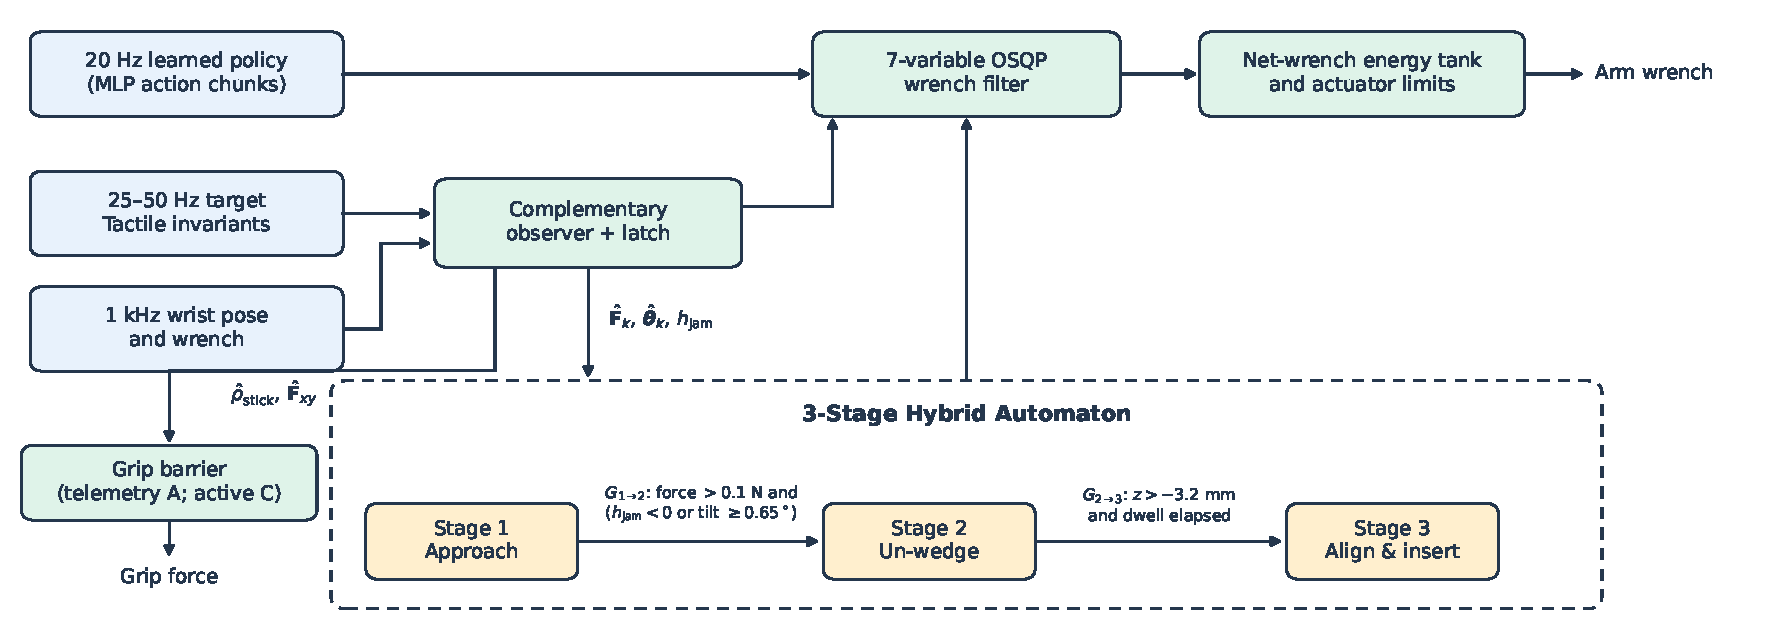
\includegraphics[width=\textwidth]{figures/controller_architecture.pdf}
\caption{Signal flow and contact-state transitions. The 25--50\,Hz tactile path is the target sensing architecture. Benchmark A supplies synthetic invariants at each simulation tick by default and uses a 50\,Hz sample-and-hold path in the perturbation sweep.}
\label{fig:architecture}
\end{figure*}

Given the 20\,Hz learned-policy wrench $\mathbf{u}_\pi$ (chunk horizon $H=\ChunkHorizon$), at 1\,kHz we solve over $\mathbf{z}=[\mathbf{u}^\top,\delta]^\top\in\mathbb{R}^7$:
\begin{equation}
\begin{aligned}
\min_{\mathbf{u},\delta}\;&\tfrac12\|\mathbf{u}-\mathbf{u}_{\mathrm{target}}\|_{\mathbf{W}}^2+\tfrac12\lambda\delta^2\\
\mathrm{s.t.}\;&\ell_z \le u_z+\delta\le r_z,\quad
 |u_x|,|u_y|\le F_{\mathrm{lat},\max},\\
& |u_z|\le 25\,\mathrm{N},\quad
|u_{4:6}|\le 6\,\mathrm{Nm},\quad |\delta|\le100\,\mathrm{N}.
\end{aligned}
\label{eq:cbf_qp}
\end{equation}
OSQP uses stage-dependent axial bounds $\ell_z,r_z$ and a signed slack. The force margin informs a feedback override and does not enter through a relative-degree-two contact model. Representative lower bounds before the force-response override are
\begin{equation}
u_{z,\mathrm{cbf}}=\begin{cases}
-F_{\mathrm{app}}-D_1\dot z, & \text{Stage 1 (free space)},\\
\ell_{\mathrm{retract}}, & \text{Stage 2},\\
-F_{\mathrm{app}}-D_3\dot z, & \text{Stage 3, low force}.
\end{cases}
\label{eq:uz_piecewise}
\end{equation}
Here $F_{\mathrm{app}}=8$\,N and the Stage 2 bound is $\ell_{\mathrm{retract}}=K_z(z_{\mathrm{clear}}-z)-D_2\dot z+\beta_f\|\hat{\mathbf F}\|+u_{f,\mathrm{delay}}$. Stage 3 holds retraction height while alignment settles, then uses an insertion law with force-dependent throttling. At \ForceTrigger\,N, an upward feedback override raises the axial lower bound. The guards are $G_{1\to2}$ with $\|\hat{\mathbf F}\|>0.1$\,N and either $h_{\mathrm{jam}}<0$ or wrist tilt $\ge0.65^\circ$, and $G_{2\to3}$ with $z>-3.2$\,mm and at least $\max(15,\tau/\Delta t)$ ticks in Stage 2 (delay rounded to ticks). Initially aligned trials can enter Stage 3 directly.

\textbf{Development-only tuning.} Stage 3 raises axial damping to \RimDamping\,Ns/m for heights between $\RimBandLower$\,mm and $-1.5$\,mm. Above $-5.8$\,mm, vertical force above 4.2\,N triggers retraction, and force above 6.5\,N latches it. During retraction and alignment the lateral centering gains are \CenterK\,N/m and \CenterD\,Ns/m. The zero-delay alignment dwell is \SettleTicks{} ticks. The axial push after passing $z=-7$\,mm is \DeepPush\,N. Stage 1 uses the learned axial reference clipped to $[-8,-6]$\,N net, and the hybrid laws determine the remaining wrench targets. The structured development panel was used to select the gains before the held-out seed was generated.

\subsection{Decoupled Grip Barrier}
\begin{equation}
F_{\mathrm{grip}}=F_{\mathrm{grip},0}+K_{\mathrm{slip}}\max(0,\rho_{\mathrm{safe}}-\hat\rho_{\mathrm{stick}})+\mu_{\mathrm{safe}}^{-1}\|\hat{\mathbf F}_{xy}\|.
\label{eq:grip_cbf}
\end{equation}
Benchmark A computes this grip demand for telemetry and uses a passive compliant peg mount. Benchmark C uses a separate simulated grip loop.

\begin{algorithm}[t]
\small
Refresh policy chunk when due and read wrist state\;
Buffer measurements and update the tactile residual\;
Advance contact stage and evaluate the force override\;
Form target wrench, axial bounds, and grip demand\;
Solve the seven-variable QP or use bounded fallback\;
Apply the tank power valve, gravity and actuator limits\;
Update tank bookkeeping from the limited wrench\;
\caption{One Benchmark A control tick ($\Delta t=1$\,ms).}
\end{algorithm}

\subsection{Safety and Passivity Arguments}
\textbf{Proposition 1 (scalar impact-arrest condition).}
For a one-dimensional elastic contact, let $d=(F_{\max}-F_g)/K$ be the remaining compression at guard force $F_g$. If the delivered net retracting force remains at least $F_r$ through compression, a sufficient condition for arrest before $F_{\max}$ is
\begin{equation}
v_0^2 \le \frac{2}{m}\left(F_rd+\frac{F_{\max}^2-F_g^2}{2K}\right).
\end{equation}
This follows by comparing kinetic energy with the work of the spring and retraction force. The simulated wrist and peg masses are 2.42 and 0.08\,kg. With $m=2.5$\,kg, $F_g=0.1$\,N, the frozen Stage 2 nominal lower bound $F_r=\RetractionFloor$\,N, $F_{\max}=15$\,N and $K=10^4$\,N/m, the scalar bound gives $v_0\le\ArrestSpeed$\,m/s. One 1\,ms sampling interval at that speed adds about \SamplingDistance\,mm of compression (about \SamplingForce\,N in the spring model), so delayed detection consumes part of the arrest margin. QP slack, tank scaling, actuator clipping, and multiple contacts can change the delivered force, limiting this calculation to the stated assumptions.

\textbf{Proposition 2 (discrete power budget).} Before actuator clipping, scaling the gravity-excluded QP wrench by $T_k$ bounds its predicted positive power by $P_{\mathrm{avail}}=(E_k-E_{\min})/\Delta t+0.8P_{\mathrm{diss}}$, with
\begin{equation}
T_k=\min(1,P_{\mathrm{avail}}/P_k),\qquad
P_k=\mathbf u_{\mathrm{QP}}^\top\mathbf v>0.
\end{equation}
Set $T_k=1$ for nonpositive power. At the floor $E_{\min}=0.05$\,J, only the dissipation credit is available. This post-solve valve scales the entire net wrench and leaves QP feasibility independent of tank energy. Stage 2 also gates delayed axial feedback when its power estimate is positive. The final update uses the clipped actuator wrench (with gravity removed) and clamps the stored energy to its allowed interval. The resulting command can differ from the QP solution, and the bookkeeping floor alone does not establish passivity of the clipped robot--environment system.

%%%%%%%%%%%%%%%%%%%%%%%%%%%%%%%%%%%%%%%%%%%%%%%%%%%%%%%%%%%%%%%%%%%%%%%%%%%%%%%%
\section{EXPERIMENTS}
\label{sec:exp}

\subsection{Simulation Setup and Idealizations}
All experiments run in MuJoCo 3.15 at 1\,kHz. The end-effector is modeled as a 6-DoF carriage coupled to a compliant in-hand peg mount (lateral stiffness $15{,}000$\,N/m, axial stiffness $30{,}000$\,N/m, rotational stiffness $80$\,Nm/rad). A Panda model is synchronized kinematically for visualization. Insertion uses the learned policy described in Appendix~\ref{app:policy}. Contour and slip use task-specific scripted references.

\textbf{Tactile idealization.} Both insertion environments synthesize opposing tapered elliptical pressure patches from the world-frame axis of the peg while loaded. Pressure goes to zero at the patch boundary, reducing grid-induced jumps in the discrete CoP. Differential CoP is calibrated to the peg axis using the same 6\,mm factor in both environments. The calibration is an analytical surrogate for asymmetric compression at the jaws, with direct access to simulated geometry. Physical deployment would need a calibrated estimator from GelSight images, such as a FEATS-style traction estimator.

\textbf{Benchmark A1 (known grasp).} We replay the \HeldN{} held-out conditions from seed \HeldSeed{} using the unified controller. The original distribution uses independent per-axis tilt in $[-15^\circ,15^\circ]$, rejecting norms above $19.2^\circ$, and independent lateral offsets in $[-0.92,0.92]$\,mm. The predefined capture basin has tilt norm at most $15^\circ$ and maximum per-axis offset at most 0.80\,mm. A1 retains its known-grasp wrench convention.

\textbf{Benchmark A2 (unknown grasp).} After freezing the code and protocol we drew seed \UnknownSeed{} and evaluated \HeldN{} random conditions once. The compliant mount has an unobserved rest tilt with uniformly sampled direction and radius from $3^\circ$ to $10^\circ$. Per-axis wrist tilts and offsets are independently uniform on $\pm4^\circ$ and $\pm0.35$\,mm. The external wrench is resolved about the wrist origin, so the moment includes the contact force lever arm. Both QPs use the same nominal wrist-to-mount geometry for lateral centering. The observer is shared. A2 uses contact-triggered entry without a free-space alignment shortcut and rim damping of \UnknownRimDamping\,Ns/m, shared by its QPs. The A2 horizon is 850\,ms. Accordingly, the within-A2 comparison controls for QP settings, while the A1-to-A2 comparison also changes the task protocol.

\textbf{Benchmark B (contour tracking).} $N=20$ phase-shifted stiff sinusoidal contours, $K_{\mathrm{env}}=10^4$\,N/m, $v_x=0.05$\,m/s, $\tau_{\mathrm{delay}}=25$\,ms.

\textbf{Benchmark C (incipient slip).} $N=20$ manipulation trials of a 0.45\,kg tool under shear pulses, $\mu\in[0.22,0.58]$.

\begin{table*}[t]
\centering
\caption{Held-out insertion comparison at 0.15\,mm clearance per side. Safe counts trials with peak force at or below 15\,N. Mean and maximum are episode peaks in newtons.}
\label{tab:bench_a}
\small
\begin{tabular}{lrrrrrrrrrr}
\toprule
& \multicolumn{5}{c}{A1: Known grasp} & \multicolumn{5}{c}{A2: Unknown in-hand tilt}\\
Controller & Insert & Jam & Safe & Mean & Max & Insert & Jam & Safe & Mean & Max\\
\midrule
\GraspComparisonRows
\bottomrule
\end{tabular}
\end{table*}

\begin{table}[t]
\centering
\caption{Benchmarks B and C ($N=\TaskTrialCount$ each).}
\label{tab:bench_bc}
\setlength{\tabcolsep}{4pt}
\begin{tabular}{lcccc}
\toprule
& \multicolumn{2}{c}{\textbf{B: contour}} & \multicolumn{2}{c}{\textbf{C: slip}}\\
\textbf{Controller} & \textbf{Safe} & \textbf{RMSE (N)} & \textbf{Drop} & \textbf{Slip (mm)}\\
\midrule
\BenchmarkBCRows
\bottomrule
\end{tabular}
\end{table}

\begin{table}[t]
\centering
\caption{Component ablations and contour peak comparisons (\AblationN{} trials per row). Force columns show mean peak, sample standard deviation, and maximum in newtons.}
\label{tab:ablation}
\setlength{\tabcolsep}{3pt}
\begin{tabular}{@{}p{0.37\columnwidth}rr@{\quad}rr@{}}
\toprule
Condition & Insert & Jam & Mean peak & Max\\
\midrule
\AblationRows
\bottomrule
\end{tabular}
\end{table}

\begin{figure*}[!t]
\centering
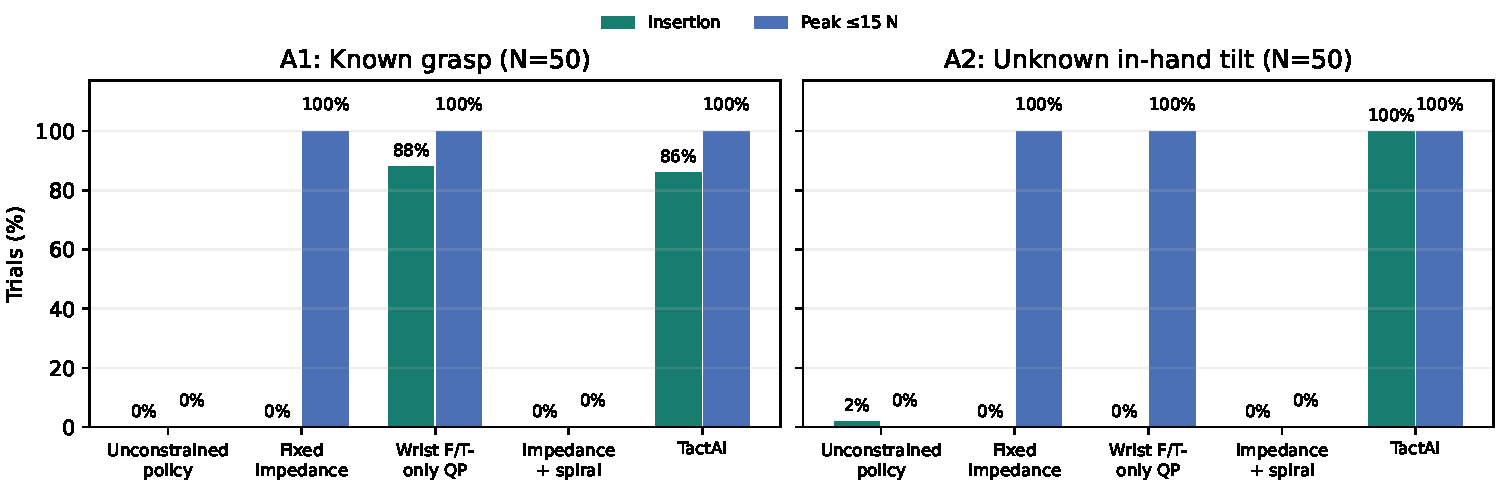
\includegraphics[width=0.92\textwidth]{figures/unified_grasp_comparison.pdf}
\caption{Insertion success and force compliance in the two held-out grasp conditions. Each percentage is computed from \HeldN{} paired conditions.}
\label{fig:bench_a}
\end{figure*}

\begin{figure*}[!t]
\centering
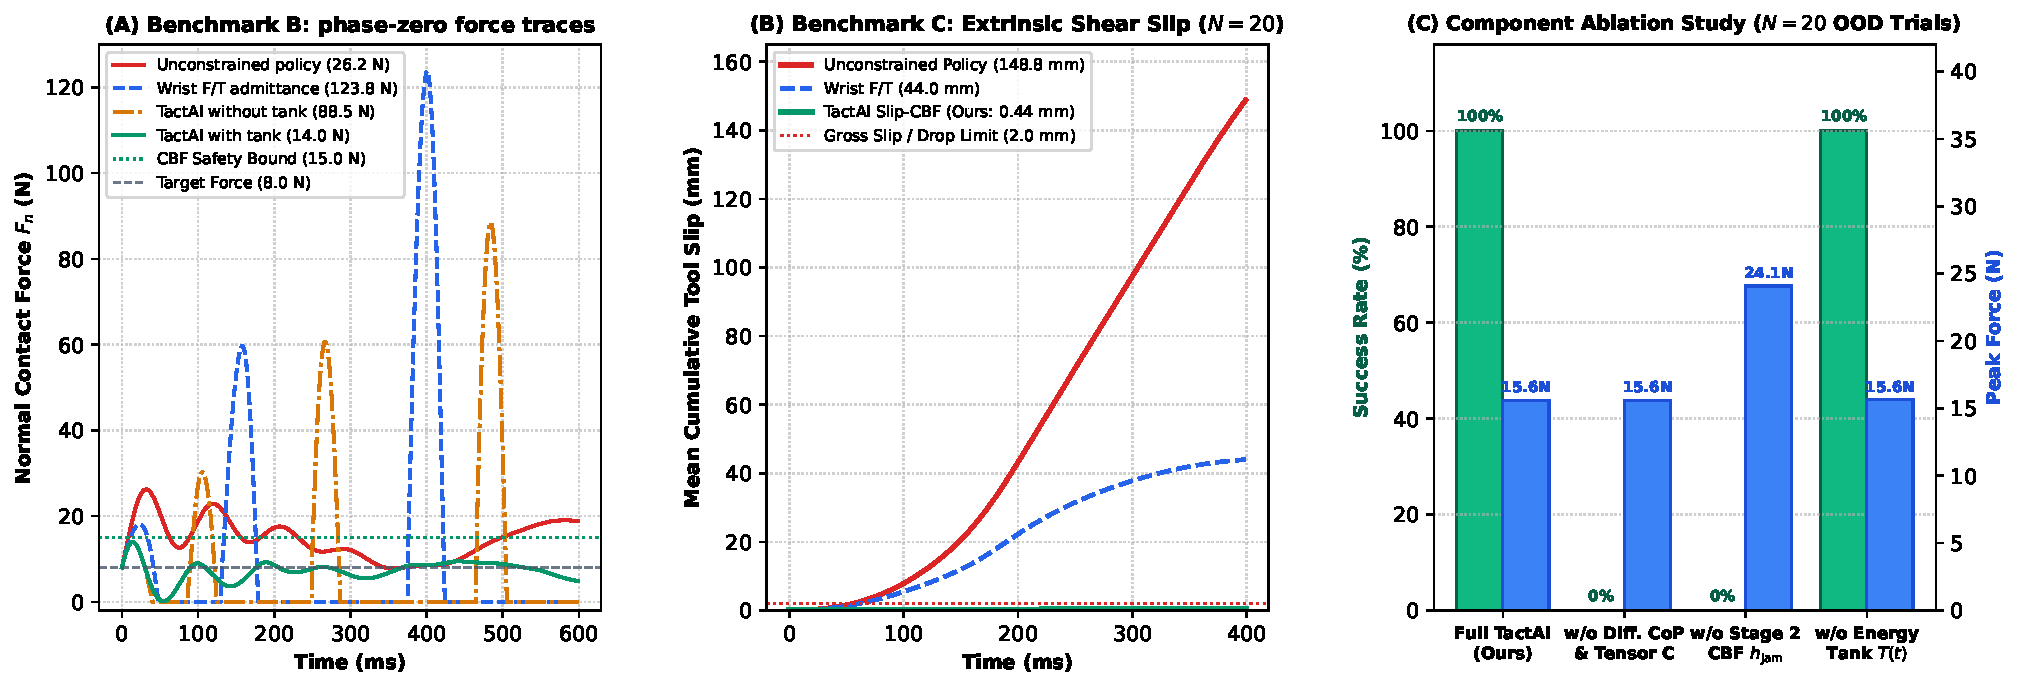
\includegraphics[width=0.95\textwidth]{figures/phase3_benchmarks_bc_ablation.pdf}
\caption{(A) Benchmark B contour force traces for the phase-zero trial. Legend peaks are computed over the displayed samples. Tables~\ref{tab:bench_bc} and~\ref{tab:ablation} summarize the full \TaskTrialCount{}-phase sweep. (B) Benchmark C cumulative slip. (C) Component ablations.}
\label{fig:bench_bc}
\end{figure*}

\subsection{Results}
On A1, TactAI inserts in \HeldInBasin{} in-basin and \HeldOutBasin{} out-of-basin trials. It records \HeldJam{} benchmark jams and \HeldSafe{} force-compliant trials. On A2, full TactAI inserts in \UnknownSuccess{} of trials, with \UnknownJam{} benchmark jams and a maximum peak of \UnknownMax\,N. The wrist-only QP remains within the force limit in \UnknownFTSafe{} A2 trials. A benchmark jam includes a simulator jam or a failed episode with peak force above 22\,N and depth below 10\,mm.

\subsection{Paired Contact Audits}
On the independent A2 development panel we perturb Gaussian CoP and stick measurements, add signed angular bias, scale the CoP-to-angle signal, and drop tactile frames. The path refreshes at 50\,Hz and holds the previous accepted frame after a drop. Of \UnknownStressN{} trials per condition, \UnknownClean{} insert at the clean 50\,Hz setting, \UnknownDropHigh{} at 30\% dropout, and \UnknownHighNoise{} under the strongest Gaussian noise. At $-1^\circ$ and $+1^\circ$ bias, successes are \UnknownBiasNegOne{} and \UnknownBiasPosOne{}, respectively. The smallest force-compliant count is \UnknownStressSafe{}, and the largest force is \UnknownStressPeak\,N.

\begin{figure*}[!t]
\centering
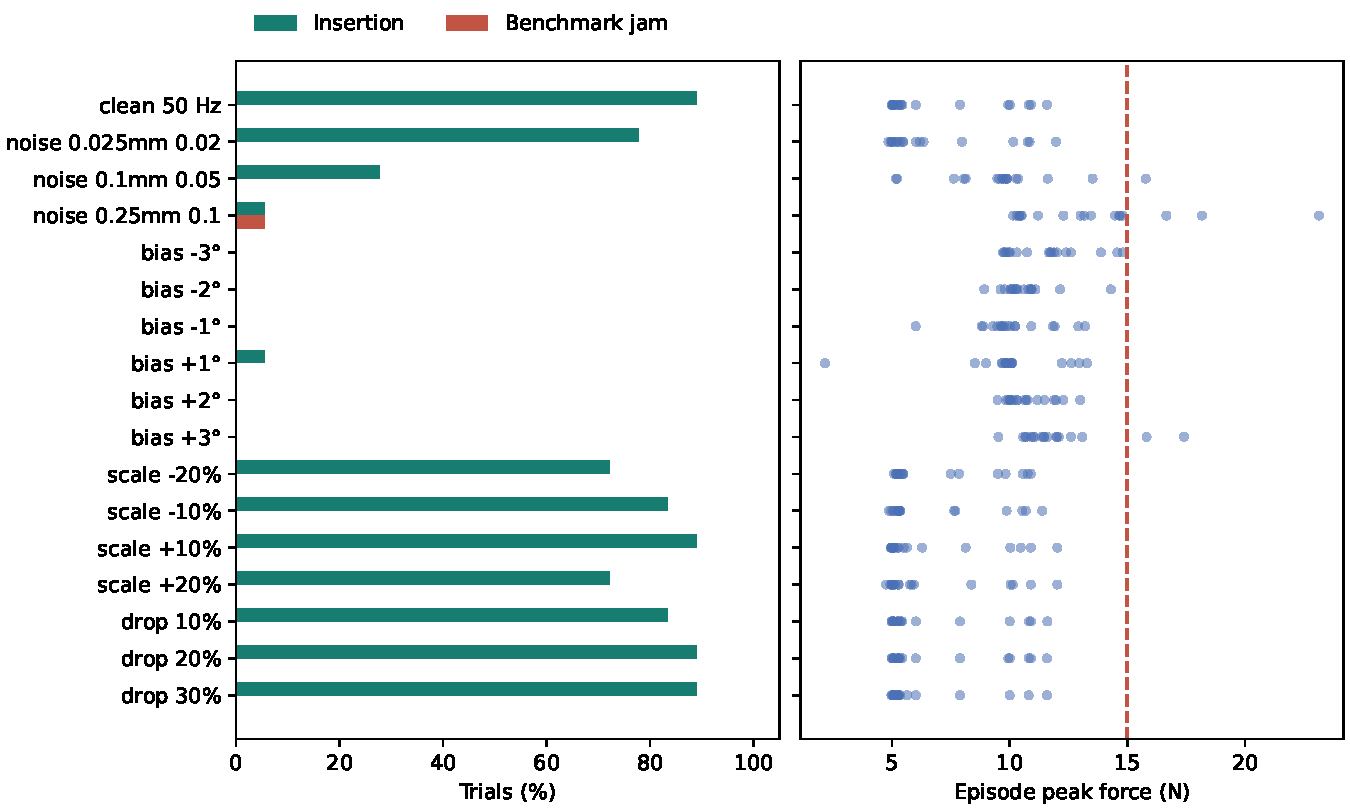
\includegraphics[width=0.84\textwidth]{figures/a2_tactile_stress.pdf}
\caption{A2 development-set tactile perturbations. Bars summarize insertion and benchmark jams. Dots are individual episode peaks, with the dashed line at 15\,N.}
\label{fig:contact_audit}
\end{figure*}

\begin{figure}[!t]
\centering
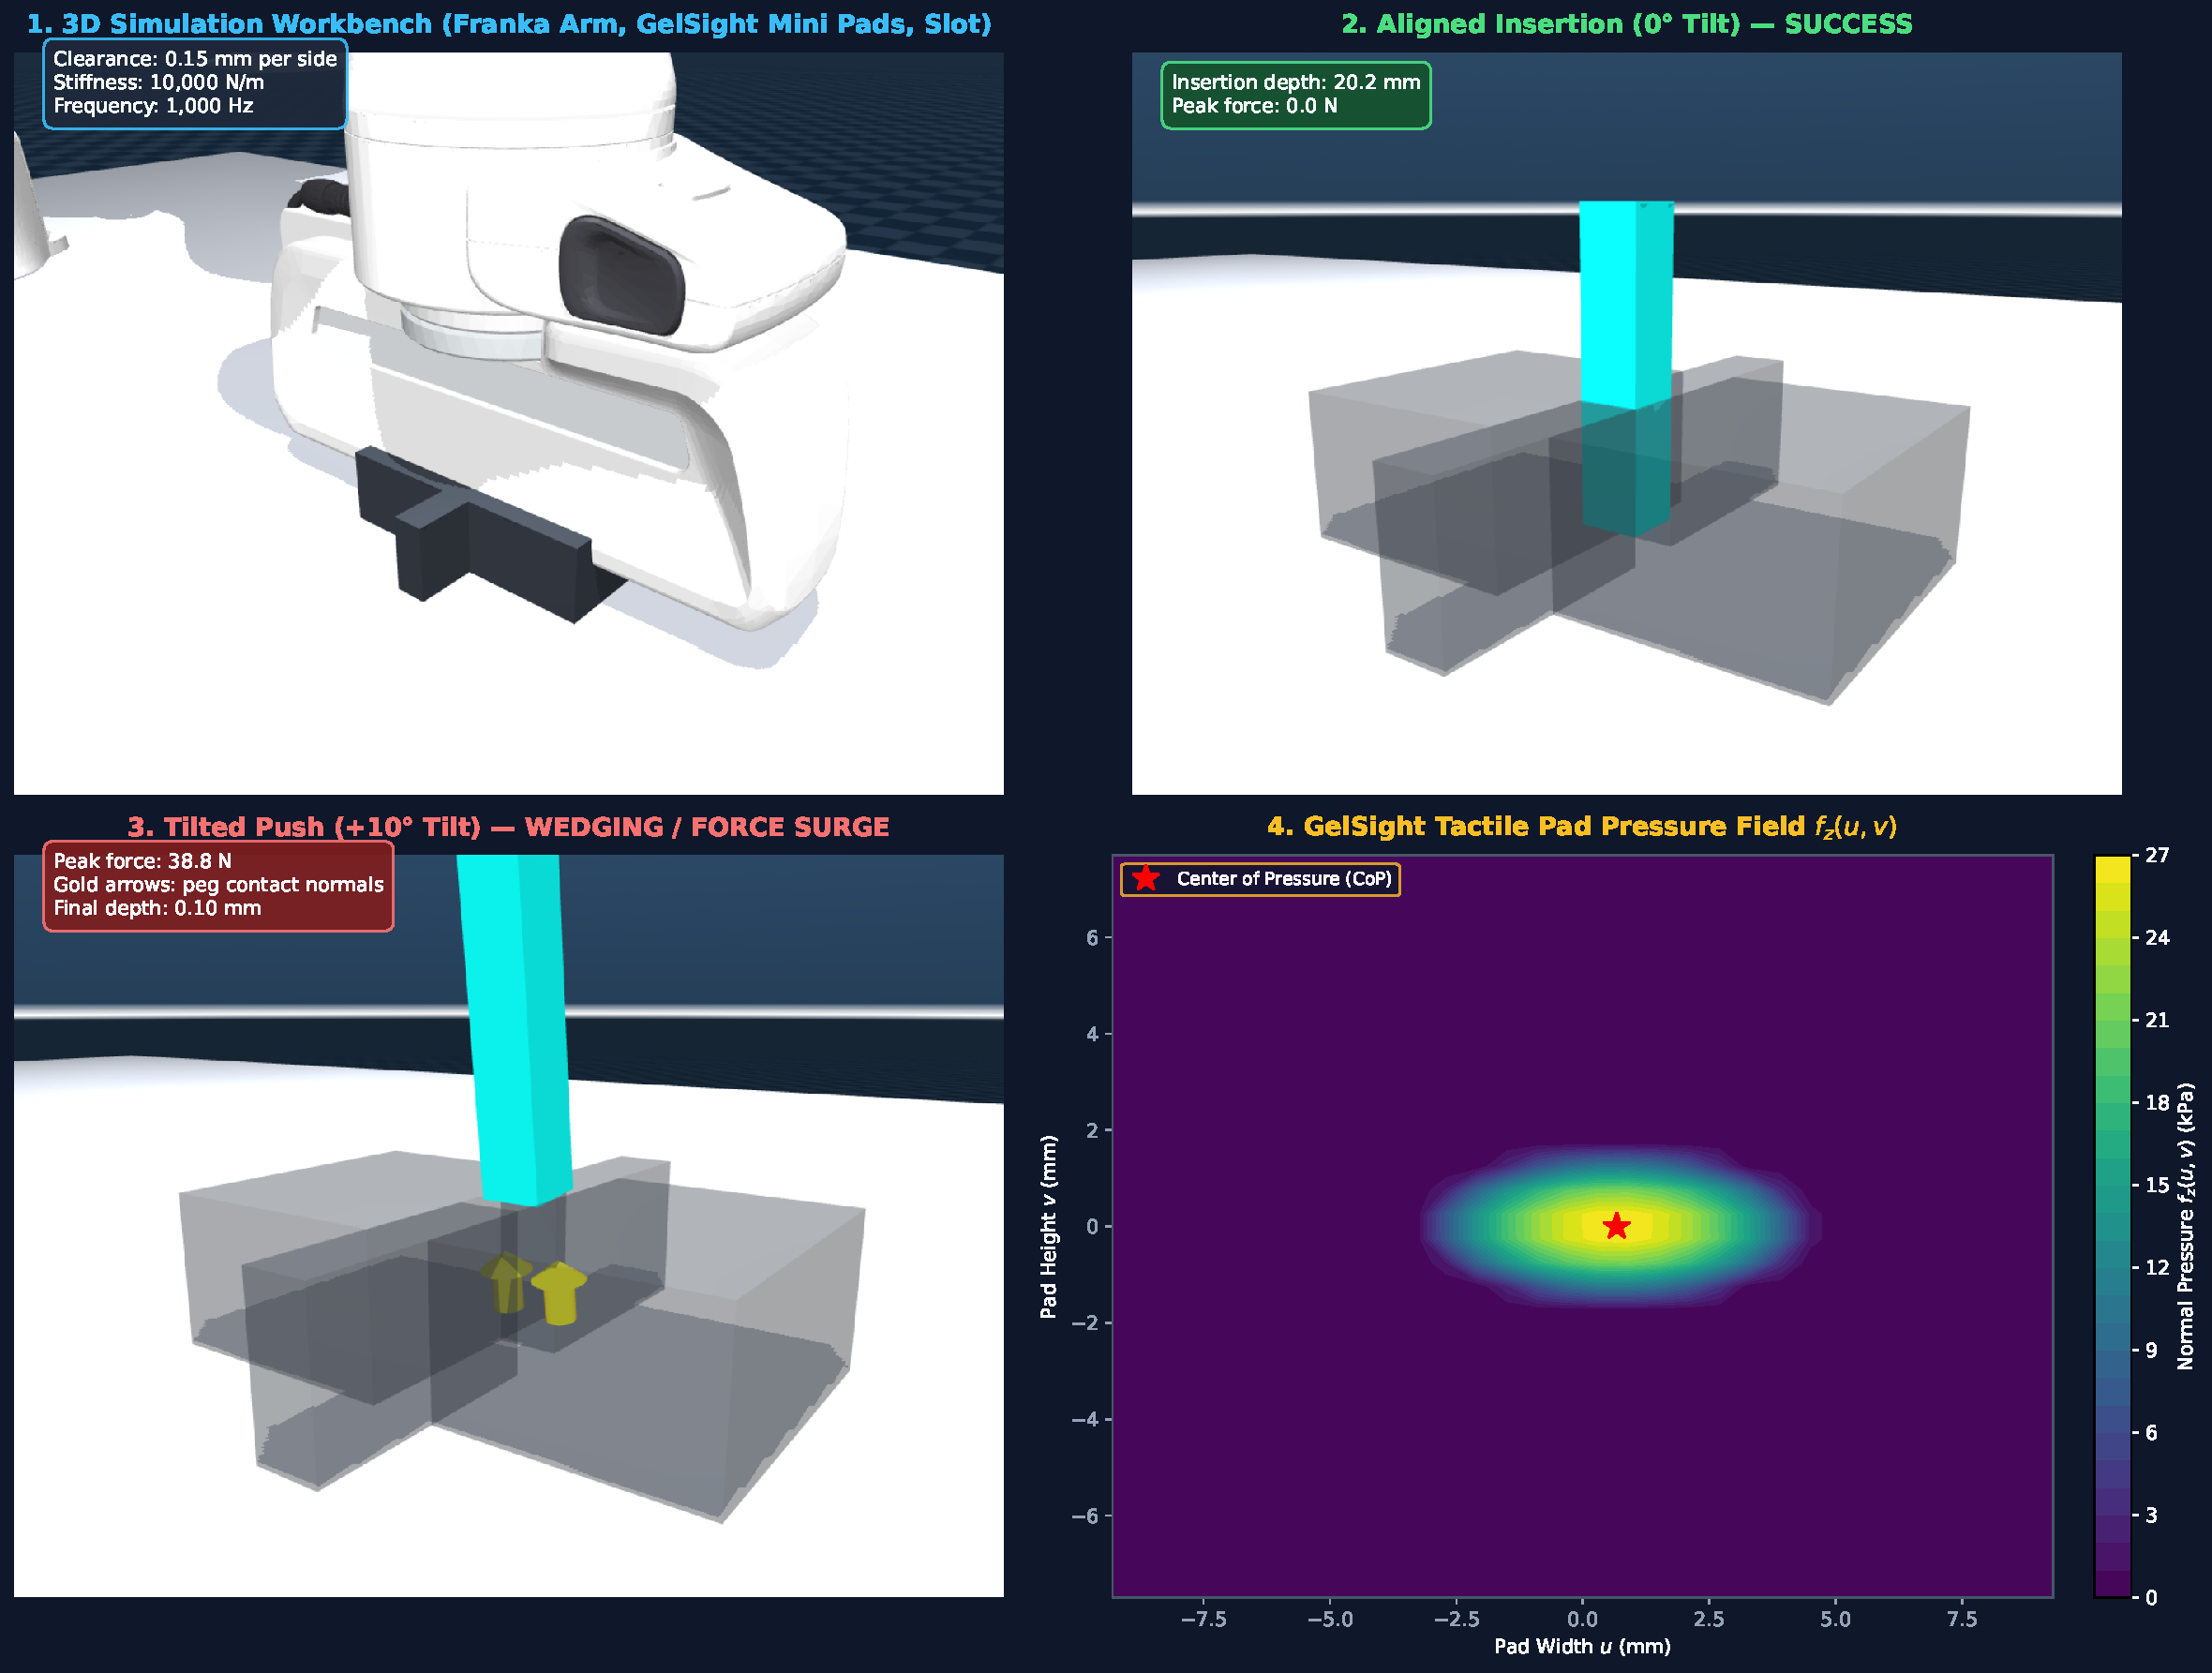
\includegraphics[width=\columnwidth]{figures/simulation_3d_overview.pdf}
\caption{MuJoCo insertion workbench. Gold arrows indicate compressive peg contact normals at wedging, with lengths chosen for visibility. The close-ups omit the decorative arm meshes. The pressure field and CoP come from the left simulated pad at that state.}
\label{fig:workbench}
\end{figure}

\begin{figure}[!t]
\centering
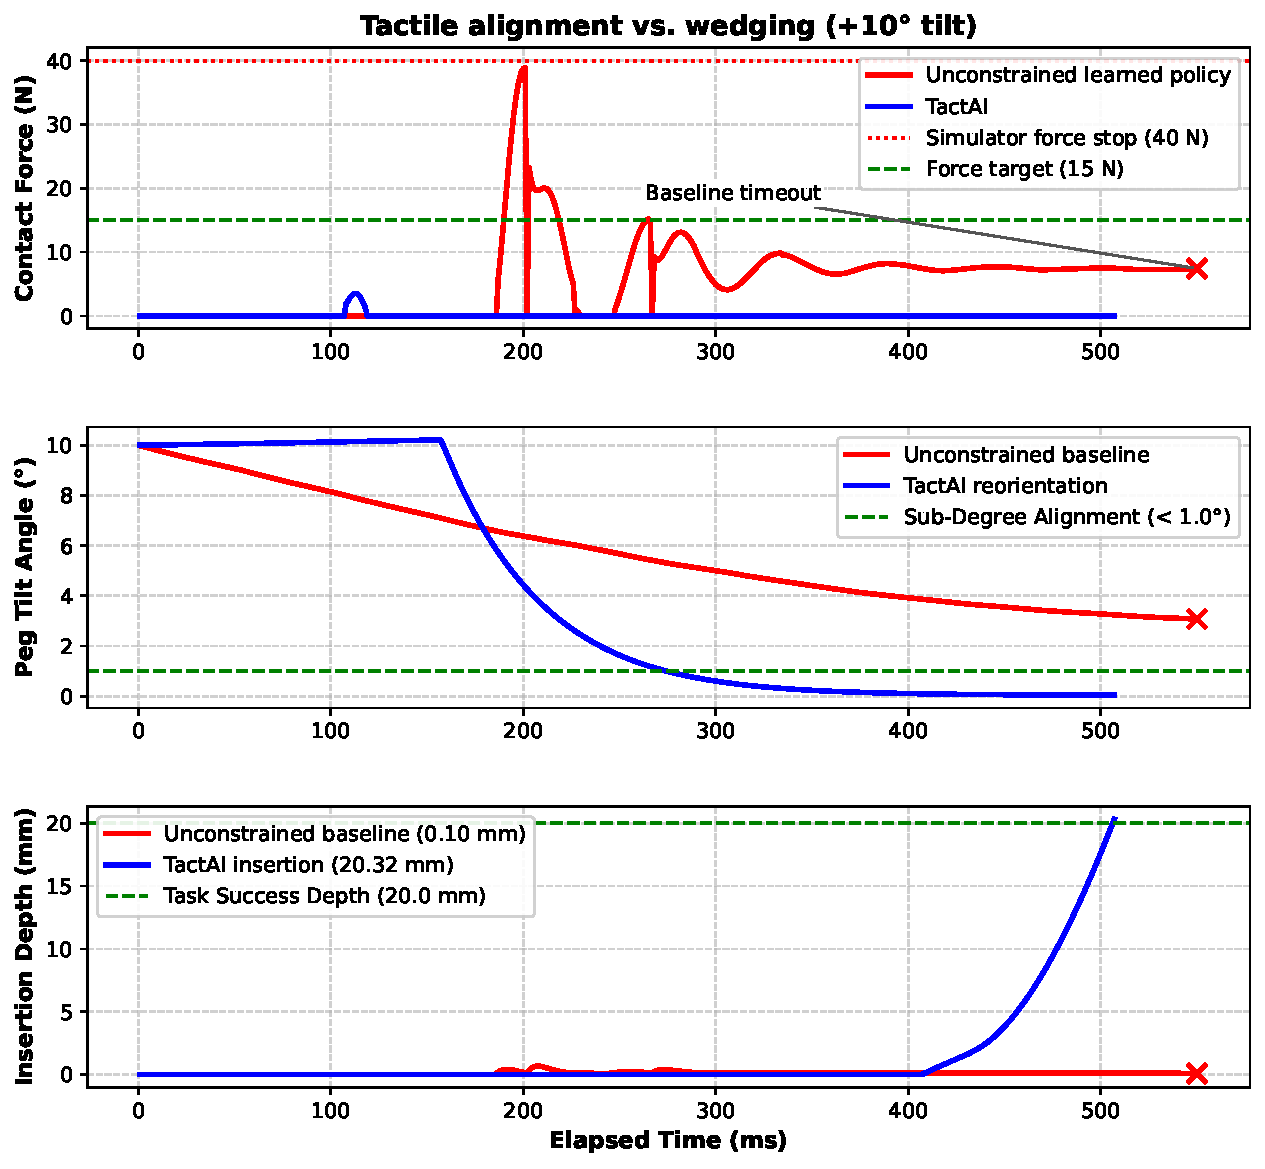
\includegraphics[width=\columnwidth]{figures/phase2_validation_benchmark.pdf}
\caption{Illustrative $\TelemetryTilt^\circ$ insertion comparison. Crosses mark the baseline \TelemetryBaselineEnd{}. Peak forces are \TelemetryBaselinePeak\,N without supervision and \TelemetryPeak\,N with TactAI.}
\label{fig:telemetry}
\end{figure}

\section{Discussion and Limitations}
The A1 results show that shared hybrid supervision accounts for most of the gain when wrist pose is a useful orientation reference. In A2, a wrist-only QP can unload the rim while leaving a crooked peg misaligned. The dual-pad estimate enables counter-tilt, separating insertion success from force compliance. In the controlled development ablation, removing proportional alignment removes the orientation target but retains damping and limited moment feedback. CoP-only and full TactAI attain the same A2 development insertion count (Table~\ref{tab:shared_ablation}).

Benchmark B isolates the effect of a tank on delayed contour tracking. Benchmark C assesses the value of stick information for retention. The A2 perturbations test dependence on the estimated grasp angle. Angle bias can remain latched throughout unloaded alignment, so small systematic errors matter even when peak force stays bounded. These are measurements on the stated simulation splits. The simulated pad has access to the true axis through its rendering model, and the wrist-origin wrench is idealized. Hardware validation requires a calibrated tactile estimator and wrist wrench acquisition with realistic delays and uncertainty.

\appendices
\section{Policy and Baselines}
\label{app:policy}

\subsection{Learned Insertion Policy}
The scripted demonstrator used measured wrist state and a nominal slot-frame goal. We sampled \DemoCount{} initial states with independent per-axis tilts within $\pm1.5^\circ$ and offsets within $\pm0.25$\,mm. The demonstrator completed \DemoSuccesses{} insertions, yielding \TrainExamples{} chunk training examples. The MLP reads 13 normalized inputs (Cartesian position and orientation, linear and angular velocity, and elapsed time). Two 64-unit tanh layers predict six wrench components over \ChunkHorizon{} ticks. The action chunk refreshes at 20\,Hz and is tracked with a fixed 1\,kHz velocity damping term (55\,Ns/m laterally, 32\,Ns/m axially, 0.45\,Nms/rad rotationally). AdamW minimizes masked mean-squared wrench error for \TrainEpochs{} epochs with batch size \TrainBatch{}, learning rate \TrainLR{}, and initialization seed \TrainSeed{}. The learned policy inserted in \NominalSuccess{} episodes from the disjoint nominal validation set and reached \UnconstrainedSuccess{} success on the fresh OOD set.

\subsection{Sensor-Driven Insertion Baselines}
The wrist F/T-only variant uses the same OSQP problem, automaton, post-solve tank, and frozen gain settings as TactAI. It evaluates $J_{\rm jam}$ from buffered wrist wrench and uses measured wrist orientation for alignment with the same external-moment feedback. The tactile residual is zero, the rotational gain is isotropic, and the absent slip measurement is assigned a neutral stick ratio of one. Neither QP reads raw peg state or switches to a special controller based on initial tilt. Fixed impedance uses translational gains 200\,N/m and 22\,Ns/m and rotational gains 4\,Nm/rad and 0.8\,Nms/rad. Its axial reference descends at 45\,mm/s and its orientation reference is the first measured wrist pose.

Impedance with spiral search triggers at $\|\mathbf F\|>1$\,N. The lateral reference has angle $2\pi(5\,\mathrm{Hz})t$ measured from contact and radius $0.15$\,mm per radian capped at 2.5\,mm. The spiral is active above $z=-10$\,mm. Lateral gains are 1400\,N/m and 40\,Ns/m, with a 12\,N componentwise limit. The axial force uses a 5\,N downward bias, 55\,Ns/m damping, and upward feedback above 6\,N vertical contact. Net axial force is clipped to $\pm12$\,N before adding 24.525\,N gravity compensation. The attitude loop uses 12\,Nm/rad and 0.7\,Nms/rad with $\pm2$\,Nm clipping.

\subsection{Wrist Comparators for Contour and Slip}
Benchmark B uses $u_z=\mathrm{clip}(-8+1.55(F_{\mathrm{delayed}}-8)-6\dot z,-25,25)$\,N with 25\,ms delay. The 2.5\,kg probe is the plant mass. In Benchmark C the wrist comparator reacts when slip velocity exceeds 4\,mm/s or displacement exceeds 0.4\,mm. Its commanded grip rises at 85\,N/s to at most 16.5\,N, from a nominal 6.5\,N.

\makeatletter
\newenvironment{auditTable}{\par\medskip\noindent\begin{minipage}{\columnwidth}
  \def\@captype{table}\centering\setlength{\tabcolsep}{3pt}}
  {\end{minipage}\par\medskip}
\makeatother
\clearpage
\section{Additional Benchmark A Results}
The following tables separate measurement, alignment, and failure outcomes. Complete per-controller failure records accompany the held-out logs.

\begin{auditTable}
\centering
\caption{Developer-panel orientation ablation. Safe counts peaks at or below 15\,N.}
\label{tab:shared_ablation}
\begin{tabular}{lp{0.34\columnwidth}rrrr}
\toprule
Panel & Controller & Insert & Jam & Safe & Max (N)\\
\midrule
\SharedAblationRows
\bottomrule
\end{tabular}
\end{auditTable}

\begin{auditTable}
\centering
\caption{Representative A2 development trial with $\ExampleGrasp^\circ$ grasp offset and $\ExampleWrist^\circ$ initial wrist roll. Final roll in degrees, peak in newtons and depth in millimeters.}
\begin{tabular}{p{.31\columnwidth}rrrrr}
\toprule
Controller & Wrist & Peg & Residual & Peak & Depth\\
\midrule
\CounterTiltRows
\bottomrule
\end{tabular}
\end{auditTable}

\begin{auditTable}
\centering
\caption{A2 held-out TactAI failures (\UnknownFailures{} total).}
\begin{tabular}{lrrl}
\toprule
Trial seed & Depth (mm) & Peak (N) & Latched\\
\midrule
\UnknownFailureRows
\bottomrule
\end{tabular}
\end{auditTable}

\begin{auditTable}
\centering
\caption{All TactAI insertion failures from the primary held-out evaluation.}
\label{tab:failure_audit}
\begin{tabular}{lllcr}
\toprule
Trial seed & Basin & End & Latch & Peak (N)\\
\midrule
\HeldFailureRows
\bottomrule
\end{tabular}
\end{auditTable}

\clearpage
\begin{thebibliography}{99}

\bibitem{helmut2025farm}
E. Helmut, N. Funk, T. Schneider, C. de Farias, and J. Peters, ``Tactile-conditioned diffusion policy for force-aware robotic manipulation,'' arXiv:2510.13324, 2025.

\bibitem{helmut2024feats}
E. Helmut, L. Dziarski, N. Funk, B. Belousov, and J. Peters, ``Learning force distribution estimation for the GelSight Mini optical tactile sensor based on finite element analysis,'' arXiv:2411.03315, 2024.

\bibitem{nguyen2024tacex}
D. H. Nguyen, T. Schneider, G. Duret, A. Kshirsagar, B. Belousov, and J. Peters, ``TacEx: GelSight tactile simulation in Isaac Sim,'' arXiv:2411.04776, 2024.

\bibitem{ames2019cbf}
A. D. Ames, S. Coogan, M. Egerstedt, G. Notomista, K. Sreenath, and P. Tabuada, ``Control barrier functions: Theory and applications,'' in \emph{Proc. European Control Conf. (ECC)}, 2019, pp. 3420--3431.

\bibitem{ferraguti2013tank}
F. Ferraguti, C. Secchi, and C. Fantuzzi, ``A tank-based approach to impedance control with variable stiffness,'' in \emph{Proc. IEEE Int. Conf. Robotics and Automation (ICRA)}, 2013, pp. 4948--4953.

\bibitem{whitney1982quasi}
D. E. Whitney, ``Quasi-static assembly of compliantly supported rigid parts,'' \emph{ASME J. Dynamic Systems, Measurement, and Control}, vol. 104, no. 1, pp. 65--77, 1982.

\bibitem{chi2023diffusion}
C. Chi, S. Feng, Y. Du, Z. Xu, E. Cousineau, B. Burchfiel, and S. Song, ``Diffusion policy: Visuomotor policy learning via action diffusion,'' in \emph{Proc. Robotics: Science and Systems (RSS)}, 2023.

\bibitem{zhao2023act}
T. Z. Zhao, V. Kumar, S. Levine, and C. Finn, ``Learning fine-grained bimanual manipulation with low-cost hardware,'' in \emph{Proc. Robotics: Science and Systems (RSS)}, 2023.


\bibitem{wabersichfilter}
K. P. Wabersich and M. N. Zeilinger, ``A predictive safety filter for learning-based control of constrained nonlinear dynamical systems,'' arXiv:1812.05506, 2018.
\bibitem{hsufilter}
K.-C. Hsu, H. Hu, and J. F. Fisac, ``The safety filter: A unified view of safety-critical control in autonomous systems,'' arXiv:2309.05837, 2023.
\bibitem{xiaohocbf}
W. Xiao and C. Belta, ``Control barrier functions for systems with high relative degree,'' arXiv:1903.04706, 2019.
\bibitem{singletarydelay}
A. Singletary, Y. Chen, and A. D. Ames, ``Control barrier functions for sampled-data systems with input delays,'' arXiv:2005.06418, 2020.
\bibitem{yuangelsight}
W. Yuan, S. Dong, and E. H. Adelson, ``GelSight: High-resolution robot tactile sensors for estimating geometry and force,'' Sensors, vol. 17, no. 12, art. 2762, 2017.
\bibitem{lambetadigit}
M. Lambeta et al., ``DIGIT: A novel design for a low-cost compact high-resolution tactile sensor with application to in-hand manipulation,'' arXiv:2005.14679, 2020.
\bibitem{dongslip}
S. Dong, W. Yuan, and E. Adelson, ``Improved GelSight tactile sensor for measuring geometry and slip,'' arXiv:1708.00922, 2017.
\bibitem{kimactive}
S. Kim and A. Rodriguez, ``Active extrinsic contact sensing: Application to general peg-in-hole insertion,'' arXiv:2110.03555, 2021.
\bibitem{kimextrinsic}
S. Kim, D. K. Jha, D. Romeres, P. Patre, and A. Rodriguez, ``Simultaneous tactile estimation and control of extrinsic contact,'' arXiv:2303.03385, 2023.
\bibitem{shecable}
Y. She, S. Wang, S. Dong, N. Sunil, A. Rodriguez, and E. Adelson, ``Cable manipulation with a tactile-reactive gripper,'' Int. J. Robot. Res., 2021, doi: 10.1177/02783649211027233.
\end{thebibliography}

\end{document}
